\chapter{Implementacja}

Założeniem projektu było stworzenie konfigurowalnej platformy umożliwiającej przeprowadzanie testów wydajnościowych dla różnych metod komunikacji międzyprocesowej. Głowna część (silnik testujący) zrealizowana została w oparciu o Javę 9 i jej wirtualną maszynę.

Dane wejściowe to m. in. wybrany sposób komunikacji oraz jego konfiguracja, a także rozmiar danych do wysłania i odbioru. Aplikacja wykona pomiary oraz zapisze wyniki w formacie CSV.

Wartość, która jest istotna to czas jaki zajęła dwukierunkowa komunikacja. Cechuje się ona nanosekundową precyzją, lecz jej rozdzielczość jest większa. Wynika to działania metody \textit{System.nanoTime()} w Javie.

\begin{lstlisting}[caption={Metoda klasy abstrakcyjnej AbstractTransferTester, która jest wykorzysywana przez wszystkie sposoby komunikacji do wykonania pomiarów (implementowane/przeciążane są ostatnie 3 metody).},captionpos=b]
    public Metrics test(TestProps testProps) {
        beforeTest(testProps);
        long start = System.nanoTime();
        try {
            execute(testProps);
        } catch (TesterException e) {
            log.error("TesterException", e);
            afterTest();
            return Metrics.error(testProps.getRequestBytes().length,
                    testProps.getResponseSize(), testType);
        }

        long time = System.nanoTime() - start;
        afterTest();
        return Metrics.of(time, testProps.getRequestBytes().length,
                testProps.getResponseSize(), testType);
    }

    protected void beforeTest(TestProps testProps) {}

    protected abstract void execute(TestProps testProps) throws TesterException;

    protected void afterTest() {}
\end{lstlisting}


Aby zachować wiarygodność testów, przeprowadzone zostały wielokrotnie - każda wykorzystana konfiguracja testowa była wykonana co najmniej 1000-krotnie.

Przed właściwym testowaniem zawsze następowały uruchomienia niepomiarowe, aby \enquote{rozgrzać maszynę writualną}. To znaczy, aby uzyskać pełną wydajność. Celem jest wcześniejsze załadowanie klas do pamięci oraz poczekanie aż JIT (ang. \textit{just-in-time compilation} - kompilacja tuż przed wykonaniem kodu) dokona kompilacji do kodu natywnego oraz optymalizacji.

Charater testów był czysto naukowy. Dane przesyłane w zapytaniach to losowe bajty oraz rozmiar oczekiwanej odpowiedzi, aby dynamicznie sterować wielkościami komunikatów - bez rekonfigurowania serwerów oczekujących na klienta.

Odpowiedź generowana po stronie implementowanej w C/C++ została ujednolicona, tak aby nie fałszować różnic między metodami transportu.

\begin{lstlisting}[caption={Fragment kodu wykorzystywanego w każdej metodzie komunikacji do generowania odpowiedzi},captionpos=b]
    for (int i = 0; i < responseSize; i++) {
        response[i] = (i % 26) + 65;
    }
\end{lstlisting}

\begin{figure}[h!]
	\centering
	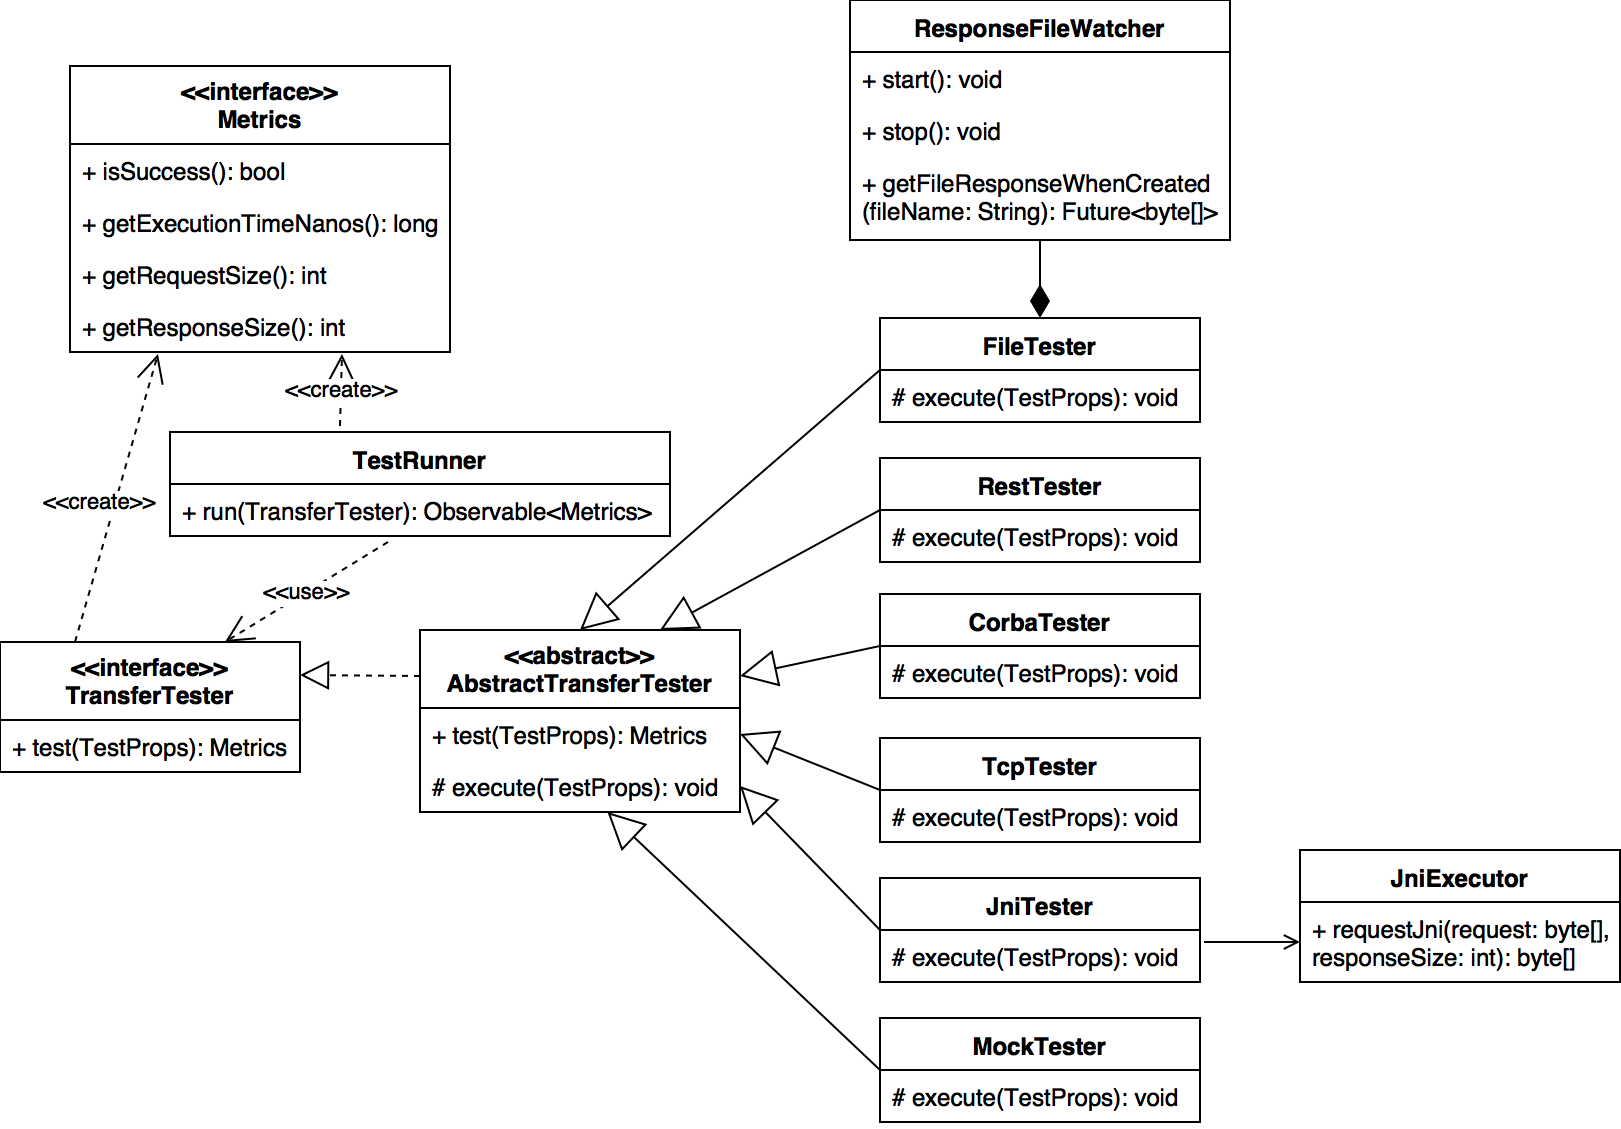
\includegraphics[width=\textwidth,height=\textheight,keepaspectratio]{img/class_diagram.png}
	\caption{Uproszczony diagram klas wykorzystany w silniku testującym.}
\end{figure}

W kolejnych sekcjach przybliżony zostanie sposób testowania poszczególnych metod komunikacji. Platformą docelową dla wszystkich implementacji jest Linux - na nim przeprowadzone zostały wszystkie uruchomienia (mimo że większość wspiera także macOS oraz Windows).

\section{Własny protokół oparty o TCP}

Zaimplementowany został własny protokół służący badaniu szybkości transferu danych oparty o gniazda TCP. Aby klient mógł zlokalizować serwer potrzebny jest mu jego adres IP i port oraz oczywiście musi istnieć możliwość stworzenia trasy.

Strona serwerowa wykorzystuje bibliotekę \texttt{unistd.h}. Klient opiera się o~standardową bibliotekę Javy, czyli klasę \texttt{java.net.Socket}.

\begin{figure}[h!]
    \centering
    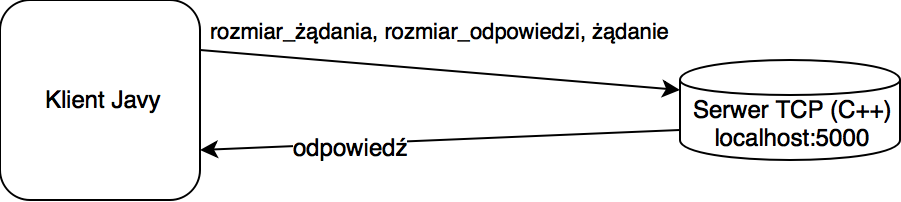
\includegraphics[width=\textwidth,height=\textheight,keepaspectratio]{img/tcp_impl_diagram.png}
    \caption{Diagram prezentujący działanie własnego protokołu opartego na TCP}
\end{figure}

Sam protokół należy do typu żądanie/odpowiedź - to znaczy za każdym razem otwierane jest gniazdo, a po otrzymaniu odpowiedzi zamykane. Jego działanie wygląda następująco:
\newline
Klient wysyła wiadomość składającą się kolejno z:
\begin{enumerate}
    \item 4 bajtów rozmiaru żądania
    \item 4 bajtów rozmiaru oczekiwanej odpowiedzi
    \item bajtów żądania w rozmiarze określonym na początku
\end{enumerate}
Serwer odpowiada bajtami odpowiedzi w rozmiarze określonym przez klienta (sam je generuje).


\section{REST}

Aby mogła zaistnieć komunikacja wykorzystująca REST, należało wcześniej wybrać format danych i~URI.

Serwer wystawia zasób pod adresem \texttt{/testResult}. Dane transferowane są w formacie JSON:
\begin{lstlisting}[caption={Format danych wysyłany przez klienta},captionpos=b]
    {
        "responseSize": 1024,
        "data": "ABCDEFGH..."
    }
\end{lstlisting}

\begin{lstlisting}[caption={Format danych zwracany przez serwer},captionpos=b]
    {
        "result": "ABCDEF..."
    }
\end{lstlisting}

\begin{figure}[h!]
    \centering
    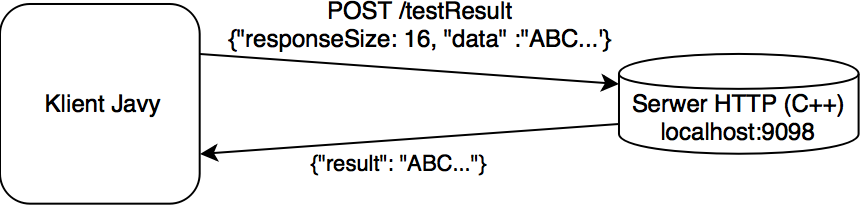
\includegraphics[width=\textwidth,height=\textheight,keepaspectratio]{img/rest_impl_diagram.png}
    \caption{Diagram prezentujący komunikację klienta z serwerem HTTP}
\end{figure}

Implemetancja strony serwerowej wykorzystuje bibliotekę ngrest (\url{https://github.com/loentar/ngrest}), służącą do tworzenie serwisów RESTowych.

Klient Javy oparty jest \textit{OkHttp} (\url{http://square.github.io/okhttp}) jako klienta HTTP oraz \textit{Jackson} \newline (\url{https://github.com/FasterXML/jackson}) do parsowania i budowania formatu JSON.


\section{Pliki}

System plików nie został stworzony w celu komunikacji typu żądanie-odpowiedź. Należało zatem zaimitować takie zachowanie. Został zaimplementowany własny protokół, który spełnia taką funkcję.

Format pliku żądania zawiera:
\newline
\texttt{rozmiar\_oczekiwanej\_odpowiedzi, bajty\_zapytania}

Rozmiar oczekiwanej odpowiedzi to 4 bajty (liczba całkowita). Plik zwrotny zawiera jedynie bajty z odpowiedzią.

Poniżej znajduje się diagram przedstawiający komunikację.

\begin{figure}[h!]
    \centering
    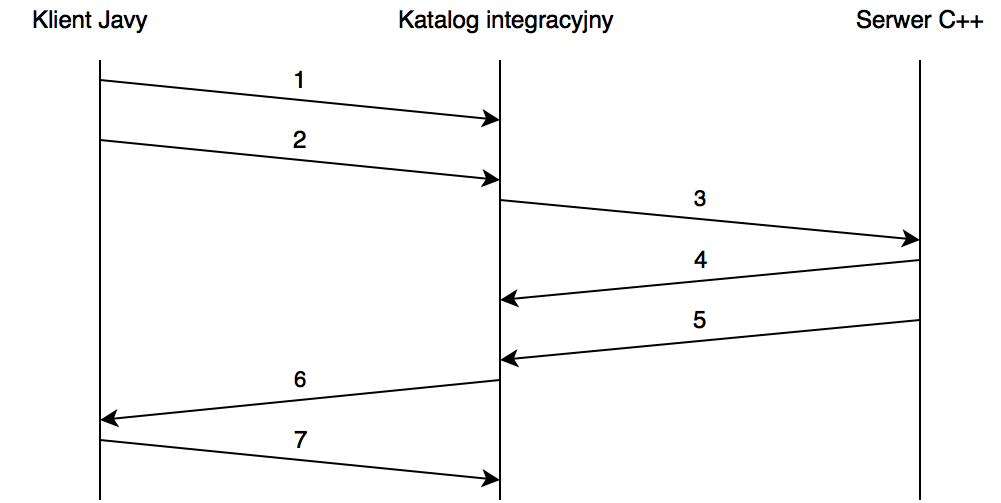
\includegraphics[width=\textwidth,height=\textheight,keepaspectratio]{img/files_impl_diagram.png}
    \caption{}
\end{figure}

\texttt{UUID} w poniższym opisie oznacza losowy ciąg znaków generowany po stronie klienta.
\begin{enumerate}
    \item Stworzenie pliku o nazwie \texttt{UUID\_request\_tmp} i zapisanie w nim żądania w formacie: 4 bajty dla rozmiaru oczekiwanej odpowiedzi, bajty żądania
    \item Zmiana nazwy stworzonego pliku na \texttt{UUID\_request}
    \item Wczytanie pliku, którego nazwa kończy się na \texttt{\_request}
    \item Stworzenie pliku o nazwie \texttt{UUID\_response\_tmp} i zapisanie w nim odpowiedzi (w żądanym rozmiarze)
    \item Zmiana nazwy pliku na \texttt{UUID\_response}
    \item Wczytanie odpowiedzi z pliku \texttt{UUID\_response}
    \item Usunięcie plików \texttt{UUID\_request} i \texttt{UUID\_response}
\end{enumerate}

W kliencie Javy zastosowany został komponent \textit{File Monitor} z biblioteki \textit{Apache Commons IO} (\url{https://commons.apache.org/proper/commons-io}). Niestety nie wspiera on natywnych interfejsów informujących o zdarzeniach w systemie plików (np. \textit{inotify} dla Linuksa, FSEvents dla macOS, czy \textit{FileSystemWatcher} dla Windowsa). Zamiast tego skonfigurowne zostało skanowanie katalogu co 2ms.

Serwer C++ wykorzystuje \textit{inotify} (podsystem jądra Linuksa, który służy do powiadamia o zdarzeniach w systemie plików \cite{inotify_man}), dzięki czemu implementacja jest wydajna i nie wykonuje zbędynch skanów katalogu.


\section{CORBA}

Aplikacje, które należy zintegrować opierając się na specyfikacji Corby, muszą skorzystać z wybranej implementacji. OmniORB jest jedną z bardziej popularnych i wydajnych. Została użyta w wersji 4 przez serwer C++. Klient wykorzystuje zaś tę dołączoną do Javy 9.

Komunikacja pomija serwis nazw - klient zna IOR, do którego wysyła zapytania.

\begin{lstlisting}[caption={Zastosowany interfejs (IDL)},captionpos=b]
    module pl {
        module kumon {
            module transfertester {
                module tester {
                    module corba {

                        interface CorbaConnector {
                            string get(in long responseSize, in string request);
                        };
                    };
                };
            };
        };
    };
\end{lstlisting}

Protokół wymiany danych informuje serwer, jakej długości jest oczekiwana odpowiedź oraz przekazuje samo żądanie. Informacja zwrotna zostaje wygenerowana tak, aby dotrzymać wymaganego rozmiaru.


\section{JNI}

Java Native Interface wymaga stworzenia pomostu między maszyną wirtualną Javy a kodem natywnym. Stworzony został interfejs komunikacji.

\begin{lstlisting}[caption={Metoda javy, która wymaga natywnej implementacji.},captionpos=b]
    public class JniExecutor {
        public native byte[] requestJni(byte[] requestBytes, int responseSize);
    }
\end{lstlisting}

Implementacja w C żądanie i oczekiwaną długość odpowiedzi, jednak są to struktury typów \texttt{jbyteArray} i \texttt{jint}, więc przed użyciem wymagają odpowiedniego mapowania. Podobnie wygląda generowanie danych zwrotnych - oczekiwany typ to \texttt{jbyteArray}.

\begin{lstlisting}[caption={Natywna implementacja w C.},captionpos=b]
    JNIEXPORT jbyteArray JNICALL Java_pl_kumon_transfertester_tester_jni_JniExecutor_requestJni(
    JNIEnv *env, jobject thisObj, jbyteArray requestBytes, jint responseSize) {

        readRequest(env, &requestBytes);
        jbyteArray response = (*env)->NewByteArray(env, responseSize);
        jbyte *bytes = prepareResponseRandomBytes(env, &response, responseSize);
        (*env)->SetByteArrayRegion(env, response, 0, responseSize, bytes);
        return response;
    }

    void readRequest(JNIEnv *env, jbyteArray* requestBytes) {
        unsigned char* buffer = (*env)->GetByteArrayElements(env, *requestBytes, NULL);
        jsize size = (*env)->GetArrayLength(env, *requestBytes);
        (*env)->ReleaseByteArrayElements(env, *requestBytes, buffer, JNI_ABORT);
    }

    jbyte* prepareResponseRandomBytes(JNIEnv *env, jbyteArray *response, jint responseSize) {
        int i;
        jbyte *bytes = (*env)->GetByteArrayElements(env, *response, 0);
        for (i = 0; i < responseSize; i++) {
            bytes[i] = (i % 26) + 65;
        }
        return bytes;
    }
\end{lstlisting}


\section{Implementacja bez komunikacji}

Ciekawy do sprawdzenia jest sam narzut platofrmy testowej, który nie wynika z generowania odpowiedzi. Aby tego dokonać, stworzony został test działający jedynie w pamięci wirtualnej maszyny Javy, który nie komunikuje się z niczym na zewnątrz.

Uniknięcie optymalizacji (aby cała pętla nie została pominięta) zostało osiągnięte przez kontrolę rozmiaru wygenerowanych danych.

\begin{lstlisting}[caption={Test sprawdzający narzut samej platformy.},captionpos=b]
    protected void execute(TestProps testProps) throws TesterException {
        byte[] mockResponse = getMockResponse(testProps.getResponseSize());
        ResponseValidator.validateLength(mockResponse, testProps);
    }

    private byte[] getMockResponse(int responseSize) {
        byte[] response = new byte[responseSize];
        for (int i = 0; i < responseSize; i++) {
            response[i] = (byte) ((i % 26) + 65);
        }
        return response;
    }
\end{lstlisting}


\section{tmp}

- wykorzystane biblioteki?
- rozmiar każdej z technologi (np. linie kodu, rozmiar)

+ testy na sucho (mock) w celu sprawdzenia narzutu samej platformy
+ obrazek architektury klientów (może per metoda komunikacji?)
+ testy powatarzane wielokrotnie, aby uniknąć skrajnych wyników
+ na początku niemierzone testy, aby rozgrzać JVM
+ snippet generowania responsa używany w C/C++
+ sekcja per metoda komunikacji (TCP, REST, komunikacja przez pliki, CORBA, JNI)

wnioski z testow:
- dokladny opis platformy (system, sprzęt)
- wykresy